\documentclass[12pt]{article}
\usepackage{homework}
\pagestyle{fancy}

% assignment information
\def\course{Statistical Mechanics}
\def\assignmentno{Problem Sheet 3}
\def\assignmentname{Gases and Black Body Radiation}
\def\name{Xin, Wenkang}
\def\time{\today}

\begin{document}

\begin{titlepage}
    \begin{center}
        \large
        \textbf{\course}

        \vfill

        \Huge
        \textbf{\assignmentno}

        \vspace{1.5cm}

        \large{\assignmentname}

        \vfill

        \large
        \name

        \time
    \end{center}
\end{titlepage}


%==========
\pagebreak
\section*{Gases and black body radiation}
%==========


\problem{3.1}{}
For particles to be distinguishable, we need to use some parameter (position, spin, colour, etc.) to label each particle and tell one from another. For example, particles in a solid with lattice structure can be distinguished by their positions. We can contrast this with an ideal gas, where particles do not have fixed positions and are indistinguishable.

In an ideal gas, we treat each particle using particle in a box model, so that they have the wave function:

\begin{equation}
    \psi(x, y, z) = A \sin{(k_{x}x)} \sin{(k_{y}y)} \sin{(k_{z}z)}
\end{equation}

where the wave numbers satisfy $k_{i} = n_{i}\pi/L_{i}$.

The energy levels are quantised according to the relation:

\begin{equation}
    E_{n_{x}, n_{y}, n_{z}} = \frac{\hbar^{2}}{2m} \left( \frac{n_{x}^{2}}{L_{x}^{2}} + \frac{n_{y}^{2}}{L_{y}^{2}} + \frac{n_{z}^{2}}{L_{z}^{2}} \right) \equiv \frac{\hbar^{2}}{2m} \mathbf{k}^{2}
\end{equation}

where we have defined the wave vector $\mathbf{k} = (k_{x}, k_{y}, k_{z})$.

We may write the partition function for a single particle as:

\begin{equation}
    \begin{split}
        Z_{1} &= \sum e^{-\beta E_{n_{x}, n_{y}, n_{z}}} \\
        &= \frac{V}{\pi^{3}} \sum \exp\left( -\beta \frac{\hbar^{2}}{2m} k^{2} \right) \frac{\pi}{L_{x}} \frac{\pi}{L_{y}} \frac{\pi}{L_{z}} \\
        &\approx \frac{V}{\pi^{3}} \int \exp\left( -\beta \frac{\hbar^{2}}{2m} k^{2} \right) \, \mathrm{d}k_{x} \mathrm{d}k_{y} \mathrm{d}k_{z} \\
        &= \frac{V}{\pi^{3}} \int \exp\left( -\beta \frac{\hbar^{2}}{2m} k^{2} \right) k^{2} \sin{\theta} \, \mathrm{d}k \mathrm{d}\theta \mathrm{d}\phi \\
        &\equiv \int_{0}^{\infty} g(k) \exp\left( -\beta \frac{\hbar^{2}}{2m} k^{2} \right) \, \mathrm{d}k \\
        &= \frac{V}{(2\pi)^{3}} \left( \frac{2\pi m}{\beta \hbar^{2}} \right)^{3/2} \\
        &\equiv \frac{V}{\lambda_{\text{th}}^{3}}
    \end{split}
\end{equation}

where we have defined the density of states $g(k) \equiv Vk^{2}/2\pi^{2}$ and the thermal wavelength $\lambda_{\text{th}} \equiv \sqrt{2\pi\hbar^{2}/m k_{B}T}$.

For a system of $N$ \mistake{non-interacting}, indistinguishable particles that sparsely populate the energy levels (i.e., each energy level is occupied by at most one particle), the partition function of the system is:

\begin{equation}
    Z = \frac{Z_{1}^{N}}{N!} = \frac{V^{N}}{\lambda_{\text{th}}^{3N} N!}
\end{equation}

\begin{correction}
    The expression is true for a system of weakly-interacting, indistinguishable particles at a high temperature so that energy levels are sparsely populated.
\end{correction}

Using Stirling's approximation, we have:

\begin{equation}
    F = -k_{B}T \ln{Z} = -Nk_{B}T \left[ \ln{\left( \frac{V}{N\lambda_{\text{th}}^{3}} \right)} + 1 \right]
\end{equation}

which leads to the entropy:

\begin{equation}
    S = -\left( \frac{\partial F}{\partial T} \right)_{V, N} = Nk_{B} \left[ \frac{5}{2} + \ln{\left( \frac{V}{N\lambda_{\text{th}}^{3}} \right)} \right]
\end{equation}

Also note the equation of state:

\begin{equation}
    P = -\left( \frac{\partial F}{\partial V} \right)_{T, N} = \frac{Nk_{B}T}{V}
\end{equation}

Consider two gases of equal temperature, volume and pressure. By the equation of state, the number of particles in each gas must be equal. Suppose that the they are made of particles of masses $m_{1}$ and $m_{2}$, and that the thermal wavelength of the first gas is $\lambda_{\text{th}, 1}$ and that of the second gas is $\lambda_{\text{th}, 2}$. Then we have the expression for their entropies:

\begin{equation}
    S_{i} = Nk_{B} \left[ \frac{5}{2} + \ln{\left( \frac{V}{N\lambda_{\text{th}, i}^{3}} \right)} \right]
\end{equation}

The action of mixing the two gases is to increase the volume of the system to $2V$, and the number of particles to $2N$. \mistake{The entropy of the mixed system becomes:}

\begin{equation}
    S_{\text{mix}} = 2Nk_{B} \left[ \frac{5}{2} + \ln{\left( \frac{V}{N\lambda_{\text{th}, f}^{3}} \right)} \right]
\end{equation}

where we define the thermal wavelength of the final system via an average particle mass:

\begin{equation}
    \lambda_{\text{th}, f} = \sqrt{\frac{2\pi\hbar^{2}}{(m_{1} + m_{2}) k_{B}T/2}}
\end{equation}

Apparently, if $m_{1} = m_{2}$, i.e., the two gases are identical (at least in term of their thermal properties), then $S_{\text{mix}} = S_{1} + S_{2}$ so that there is no entropy change upon mixing. \mistake{If, however, $m_{1} \neq m_{2}$, we need to compare:}

\begin{equation}
    \begin{split}
        \Delta S &= S_{\text{mix}} - S_{1} - S_{2} \\
        &= Nk_{B} \left[ -2\ln{\left( \frac{V}{N\lambda_{\text{th}, f}^{3}} \right)} + \ln{\left( \frac{V}{N\lambda_{\text{th}, 1}^{3}} \right)} + \ln{\left( \frac{V}{N\lambda_{\text{th}, 2}^{3}} \right)} \right] \\
        &= Nk_{B} \ln{\left( \frac{\lambda_{\text{th}, f}^{6}}{\lambda_{\text{th}, 1}^{3}\lambda_{\text{th}, 2}^{3}} \right)} \\
        &= 3Nk_{B} \ln{\left[ \frac{\sqrt{m_{1}m_{2}}}{(m_{1} + m_{2})/2} \right]}
    \end{split}
\end{equation}

The function inside the logarithm has maximum of unity along the line $m_{1} = m_{2}$, so that $\Delta S \geq 0$ for any $m_{1} \neq m_{2}$. There is an increase in entropy upon mixing two gases of different masses since information about the identity of the particles is lost in the process.

\begin{correction}
    The entropy of the mixed system becomes:

    \begin{equation}
        S_{\text{mix}} = Nk_{B} \left[ \frac{5}{2} + \ln{\left( \frac{2V}{N\lambda_{\text{th}, 1}^{3}} \right)} \right] + Nk_{B} \left[ \frac{5}{2} + \ln{\left( \frac{2V}{N\lambda_{\text{th}, 2}^{3}} \right)} \right]
    \end{equation}

    If $m_{1} \neq m_{2}$, we need to compare:

    \begin{equation}
        \begin{split}
            \Delta S &= S_{\text{mix}} - S_{1} - S_{2} \\
            &= Nk_{B} \left[ \ln{\left( \frac{2V}{N\lambda_{\text{th}, 1}^{3}} \right)} + \ln{\left( \frac{2V}{N\lambda_{\text{th}, 2}^{3}} \right)} - \ln{\left( \frac{V}{N\lambda_{\text{th}, 1}^{3}} \right)} - \ln{\left( \frac{V}{N\lambda_{\text{th}, 2}^{3}} \right)} \right] \\
            &= 2Nk_{B} \ln{2}
        \end{split}
    \end{equation}

    which agrees with results from Joule expansion.
\end{correction}
\qed


\problem{3.2}{}

\subproblem{i}
Treating the nitrogen gas as an ideal diatomic gas, we have the single-particle partition function:

\begin{equation}
    Z_{1} = Z_{\text{trans}} Z_{\text{vib}} Z_{\text{rot}}
\end{equation}

By equipartition theorem, the heat capacity of the gas approaches $C_{V} = 7k_{B}/2$ at high temperature. In the temperature range $T_{r} < T < T_{v}$, the heat capacity increases from $5k_{B}/2$ to $7k_{B}/2$ as the vibrational modes become excited. From the data given, we have approximately $T_{r} = \qty{170}{K}$. In this range, the increase in $C_{V}$ is mostly explained by the vibrational modes, which gives the heat capacity:

\begin{equation}
    C_{V,\text{vib}} = k_{B} \left( \frac{\hbar \omega}{k_{B}T} \right)^{2} \frac{\exp\left( \hbar \omega/k_{B}T \right)}{\left[ \exp\left( \hbar \omega/k_{B}T \right) - 1 \right]^{2}}
\end{equation}

We may fit the given data (with $C/Nk_{B}$ off set by $5/2$) to the function of the form:

\begin{equation}
    \left( A/T^{2} \right) \frac{\exp\left( A/T \right)}{\left[ \exp\left( A/T \right) - 1 \right]^{2}}
\end{equation}

where $A$ is a fitting parameter evaluated to be $\qty{3196.93}{K}$.

This gives an estimate for the vibrational frequency of nitrogen gas:

\begin{equation}
    \omega = \frac{k_{B}A}{\hbar} = \qty{4.19e14}{rads^{-1}}
\end{equation}

\begin{figure}[h]
    \centering
    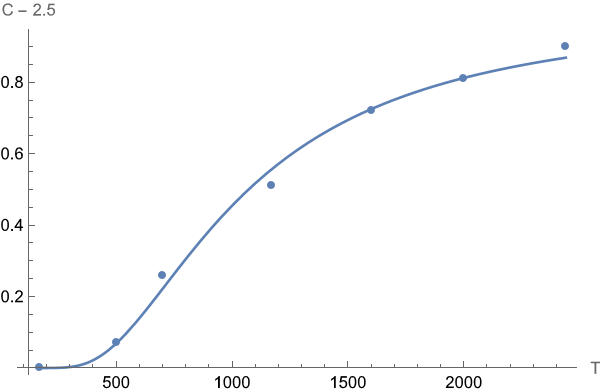
\includegraphics[width=0.6\textwidth]{../plots/statistics_3_2_a.png}
    \caption{Data with fitted curve for the heat capacity of nitrogen gas.}
\end{figure}

\subproblem{ii}
The bond length of nitrogen molecule is of unity order in angstroms, that is, $\qty{1}{\angstrom} = \qty{1e-10}{m}$. This means that the characteristic temperature for the rotational modes is:

\begin{equation}
    \theta_{\text{rot}} = \frac{\hbar^{2}}{2I k_{B}} = \frac{\hbar^{2}}{4mR^{2} k_{B}} = \frac{\hbar^{2}}{mD^{2} k_{B}} \approx \qty{3.5}{K}
\end{equation}

This means that it is possible to freeze out rotational and vibrational modes of nitrogen gas as long as the temperature can be lowered to unity order, which is easily attainable in a laboratory setting. \mistake{In fact, the space has a temperature around $\qty{2.7}{K}$}.

\begin{correction}
    But at this temperature, nitrogen already exists as a liquid, so it is not possible to freeze out the rotational and vibrational modes.
\end{correction}
\qed


\problem{3.3}{}
In the range $\theta_{\text{rot}} \ll T \ll \theta_{\text{vib}}$, the single-particle partition function of a diatomic gas is:

\begin{equation}
    Z_{1} = \left( \frac{V}{\lambda_{\text{th}}^{3}} \right) \left( \frac{T}{2  \theta_{\text{rot}}} \right) \frac{\exp\left( -\theta_{\text{vib}}/2T \right)}{1 - \exp\left( -\theta_{\text{vib}}/2T \right)}
\end{equation}

where the last term does not vary much with temperature as long as $T \ll \theta_{\text{vib}}$.

Since $\lambda_{\text{th}} \propto T^{-1/2}$, we see that $Z_{1} \propto VT^{5/2}$. In this regime, the free energy is:

\begin{equation}
    F_{1} = -k_{B}T \ln{Z_{1}} \propto -\frac{5}{2} T \ln{(V^{2/5}T)}
\end{equation}

and the entropy is:

\begin{equation}
    S_{1} = -\left( \frac{\partial F_{1}}{\partial T} \right)_{V} \propto \frac{5}{2} \ln{(V^{2/5}T)} \propto \ln{(VT^{5/2})}
\end{equation}

Therefore, along an adiabat, we need $VT^{5/2}$ to be constant. But the equation of state is:

\begin{equation}
    P = -\left( \frac{\partial F_{1}}{\partial V} \right)_{T} \propto \frac{T}{V}
\end{equation}

We can then replace $T$ with $PV$ to demand that $V^{7/2} P^{5/2}$ is constant, which is equivalent to:

\begin{equation}
    PV^{7/5} = \text{const}
\end{equation}
\qed


\problem{3.4}{}
The Gibbs function can be written as:

\begin{equation}
    G = U - TS + PV = F + PV = F - V \left( \frac{\partial F}{\partial V} \right)_{T}
\end{equation}

This means that $G$ can be expressed in terms of the partition function as:

\begin{equation}
    G = k_{B}T \left[ V \left( \frac{\partial \ln{Z}}{\partial V} \right)_{T} - \ln{Z} \right]
\end{equation}

For an ideal gas, this becomes:

\begin{equation}
    G = F + PV = F + Nk_{B}T
\end{equation}
\qed


\problem{3.5}{}
We treat photons as a group of spin-one bosons who are not allowed to have zero spin. Since photons are not conserved, we set the chemical potential to zero. The density of states in $k$-space is:

\begin{equation}
    g(k) \, \mathrm{d}k = (2s + 1) \frac{V}{(2\pi)^{3}} 4\pi k^{2} \, \mathrm{d}k = \frac{V}{\pi^{2}} k^{2} \, \mathrm{d}k
\end{equation}

where we replace the spin degeneracy factor $(2s + 1)$ with two since zero spin is not allowed.

Transforming to $\omega$-space, we have:

\begin{equation}
    g(\omega) \, \mathrm{d}\omega = \frac{V}{\pi^{2}} \frac{\omega^{2}}{c^{3}} \, \mathrm{d}\omega
\end{equation}

We know that the energy of a photon is given by $E_{\omega} = \hbar \omega$ and the occupation number of a mode is:

\begin{equation}
    n_{\omega} = \frac{1}{\exp\left( \beta \hbar \omega \right) - 1}
\end{equation}

This means we can write the internal energy as:

\begin{equation}
    \frac{U}{V} = \frac{1}{V} \int_{0}^{\infty} g(\omega) E_{\omega} n_{\omega} \, \mathrm{d}\omega \equiv \int_{0}^{\infty} \rho_{\omega} \, \mathrm{d}\omega
\end{equation}

where we define the spectral energy density:

\begin{equation}
    \rho_{\omega} \equiv \frac{\hbar}{\pi^{2}c^{3}} \frac{\omega^{3}}{\exp\left( \beta \hbar \omega \right) - 1}
\end{equation}

The maximum of $\rho_{\omega}$ can be numerically found to be $2.82 k_{B}T/\hbar$. We can also define the number density of photons:

\begin{equation}
    n_{\omega} \equiv \frac{1}{V} g(\omega) \frac{1}{\exp\left( \beta \hbar \omega \right) - 1} = \frac{1}{\pi^{2}c^{3}} \frac{\omega^{2}}{\exp\left( \beta \hbar \omega \right) - 1}
\end{equation}

whose maximum is at $1.59 k_{B}T/\hbar$.
\qed


\problem{3.6}{}
Instead of treating the photons as a gas of bosons, we can treat them as a collection of harmonic oscillators. The single-particle partition function is:

\begin{equation}
    Z_{1} = \frac{1}{1 - \exp\left( -\beta \hbar \omega \right)} = \frac{1}{1 - \exp\left( -h\nu/k_{B}T \right)}
\end{equation}

where we have ignored the zero-point energy.

\subproblem{i}
For a collection of $N$ non-interacting harmonic oscillators each labelled by a frequency $\nu_{j}$, the partition function is:

\begin{equation}
    \ln{Z} = \sum_{j} \ln{Z_{j}} = -\sum_{j = 1}^{\infty} \ln{\left[ 1 - \exp\left( -h \nu_{j}/k_{B}T \right) \right]}
\end{equation}

If $\nu_{j}$ are very closely spaced, we can replace the sum with an integral:

\begin{equation}
    \ln{Z} = -\int_{0}^{\infty} g(\nu) \ln{\left[ 1 - \exp\left( -h \nu/k_{B}T \right) \right]} \, \mathrm{d}\nu
\end{equation}

where we define the density of states $g(\nu) \, \mathrm{d}\nu$ as the number of modes in the frequency range $\nu$ to $\nu + \mathrm{d}\nu$.

\subproblem{ii}
For photons, the energy levels depend on the frequency $\nu$ via $E = h \nu$. On the other hand, the wave numbers of photons are quantised according to boundary conditions:

\begin{equation}
    k_{i} = \frac{2\pi \nu_{i}}{c} = \frac{\pi}{L_{i}} n_{i}
\end{equation}

which means that the frequency levels are quantised as:

\begin{equation}
    \nu_{i} = \frac{c}{2L_{i}} n_{i}
\end{equation}

with the smallest frequency change $\Delta \nu_{i} = c/2L_{i}$.

We can then write the sum as an integral:

\begin{equation}
    \begin{split}
        \ln{Z} &= -2 \sum_{j = 1}^{\infty} \ln{\left[ 1 - \exp\left( -h \nu_{j}/k_{B}T \right) \right]} \\
        &= -2 \left( \frac{8L_{x}L_{y}L_{z}}{c^{3}} \right) \sum_{j = 1}^{\infty} \ln{\left[ 1 - \exp\left( -h \nu_{j}/k_{B}T \right) \right]} \Delta \nu_{x} \Delta \nu_{y} \Delta \nu_{z} \\
        &\approx -16\frac{V}{c^{3}} \int \ln{\left[ 1 - \exp\left( -h \nu/k_{B}T \right) \right]} \, \mathrm{d}^{3}\nu \\
        &= -16\frac{V}{c^{3}} \int_{0}^{\pi/2} \int_{0}^{\pi/2} \int_{0}^{\infty} \ln{\left[ 1 - \exp\left( -h \nu/k_{B}T \right) \right]} \nu^{2} \sin{\theta} \, \mathrm{d}\nu \mathrm{d}\theta \mathrm{d}\phi \\
        &= -\frac{8\pi V}{c^{3}} \int_{0}^{\infty} \ln{\left[ 1 - \exp\left( -h \nu/k_{B}T \right) \right]} \nu^{2} \, \mathrm{d}\nu
    \end{split}
\end{equation}

where the extra factor of 2 comes from the two polarisations of the photon.

\subproblem{iii}
The internal energy is:

\begin{equation}
    U = -\left( \frac{\partial \ln{Z}}{\partial \beta} \right)_{V} = \frac{8\pi V}{c^{3}} \int_{0}^{\infty} \frac{h \nu^{3} \exp\left( -h \nu/k_{B}T \right)}{1 - \exp\left( -h \nu/k_{B}T \right)} \, \mathrm{d}\nu
\end{equation}

Consider the change of variable $x \equiv h\nu/k_{B}T$, we have:

\begin{equation}
    \begin{split}
        U &= \frac{8\pi V}{c^{3}} h \left( \frac{k_{B}T}{h} \right)^{4} \int_{0}^{\infty} \frac{x^{3}}{e^{x} - 1} \, \mathrm{d}x \\
        &= \frac{8\pi V}{c^{3}} h \left( \frac{k_{B}T}{h} \right)^{4} \frac{\pi^{4}}{15} \\
        &= \frac{8\pi^{5} (k_{B}T)^{4}}{15c^{3} h^{3}} V
    \end{split}
\end{equation}

\subproblem{iv}
Returning to the expression for $\ln{Z}$, we can use integration by parts to write:

\begin{equation}
    \begin{split}
        \ln{Z} &= -\frac{8\pi V}{c^{3}} \int_{0}^{\infty} \ln{\left[ 1 - \exp\left( -h \nu/k_{B}T \right) \right]} \nu^{2} \, \mathrm{d}\nu \\
        &= -\frac{8\pi V}{c^{3}} \left[ \left. \frac{1}{3} \nu^{3} \ln{\left[ 1 - \exp\left( -h \nu/k_{B}T \right) \right]} \right|_{0}^{\infty} - \frac{1}{3} \int_{0}^{\infty} \frac{(h/k_{B} T) \nu^{3} \exp\left( -h \nu/k_{B}T \right)}{1 - \exp\left( -h \nu/k_{B}T \right)} \, \mathrm{d}\nu \right] \\
        &= \frac{8\pi V}{c^{3}} \frac{1}{3k_{B} T} \int_{0}^{\infty} \frac{h \nu^{3} \exp\left( -h \nu/k_{B}T \right)}{1 - \exp\left( -h \nu/k_{B}T \right)} \, \mathrm{d}\nu \\
        &= \frac{1}{3k_{B} T} U \\
        &= \frac{8\pi^{5} (k_{B}T)^{3}}{45c^{3} h^{3}} V
    \end{split}
\end{equation}

The equation of state is then:

\begin{equation}
    P = -\left( \frac{\partial F}{\partial V} \right)_{T} = k_{B}T \left( \frac{\partial \ln{Z}}{\partial V} \right)_{T} = \frac{1}{3} \frac{U}{V} = \frac{8\pi^{5} (k_{B}T)^{4}}{45c^{3} h^{3}}
\end{equation}

where we identify the Stefan's constant $\sigma = 8\pi^{5} k_{B}^{4}/(15c^{3} h^{3})$.
\qed


\problem{3.7}{}
At $T = \qty{2e7}{K}$, the radiation pressure is:

\begin{equation}
    P = \frac{4\sigma}{3c} T^{4} = \qty{4.03e13}{N/m^{2}} = \qty{4.03e8}{atm}
\end{equation}

which is only $0.1\%$ of the gas pressure at the centre of the sun.
\qed


\end{document}